\documentclass{article}

% ---------------------------------------------------------------------------------------------------------------
% Build:  pdflatex main && bibtex main && pdflatex main && pdflatex main
% Anonymous submission (default) or named preprint: set \preprinttrue below.
% ---------------------------------------------------------------------------------------------------------------
\newif\ifpreprint
\preprintfalse
\ifpreprint
  \usepackage[preprint]{neurips_2025}
\else
  \usepackage{neurips_2025}
\fi
% The official style names NeurIPS 2025 in the submission footer; the target is the next NeurIPS.
% Replace neurips_2025.sty with the official file of the target year when it is released, then delete these lines.
\makeatletter
\renewcommand{\@neuripsordinal}{41st}
\renewcommand{\@neuripsyear}{2027}
\makeatother

\usepackage[utf8]{inputenc}
% \usepackage[T1]{fontenc}  % off here: without cm-super it embeds bitmap (Type 3) fonts; fine to re-enable on a full TeX Live
\usepackage{hyperref}
\usepackage{float}
\usepackage{url}
\usepackage{booktabs}
\usepackage{amsfonts,amsmath}
\usepackage{nicefrac}
\usepackage{microtype}
\usepackage{xcolor}
\usepackage{graphicx}
\usepackage{multirow}
\usepackage{tabularx}
\usepackage{tikz}
\usetikzlibrary{positioning,arrows.meta,fit,calc}
\usepackage{caption}
\captionsetup{font=small,labelfont=bf}
\usepackage{enumitem}
\setlist{leftmargin=1.3em,itemsep=1pt,topsep=2pt}

\definecolor{atlasblue}{HTML}{1F5FBF}
\hypersetup{colorlinks=true,linkcolor=atlasblue!75!black,citecolor=atlasblue!75!black,urlcolor=atlasblue!75!black}
\newcommand{\pmu}{\ensuremath{\mu\mathrm{g/m^3}}}
\newcommand{\pmtf}{PM$_{2.5}$}
\newcommand{\trk}[1]{\textsc{#1}}

\title{Small Sensor-Only Models Beat Time-Series Foundation Models on Indian Air Quality: A Pre-Registered Evaluation}

\ifpreprint
\author{%
  Aditya Kumar \qquad Anupam Singh\\
  ParadoxAI Lab\\
  \texttt{contact.paradoxailab@gmail.com}
}
\else
\author{Anonymous Author(s)\\Affiliation\\Address\\\texttt{email}}
\fi

\begin{document}
\maketitle

\begin{abstract}
Time-series foundation models (TSFMs) forecast unseen series zero-shot and lead public benchmarks. We ask whether a
small model trained only on Indian monitoring-station data can beat them at the task those stations exist for:
forecasting \pmtf{} for the next 24 hours. We present \emph{Atlas}, a 0.97M-parameter spatio-temporal forecaster with
graph-biased attention across stations and latent dynamics driven by known future inputs, and evaluate it under a
protocol in which every rule was committed to a public repository before the score it governs, and every comparison
is a Diebold--Mariano test, run separately on stations used in training and on stations never used. On an all-India
test that no model choice ever touched (14 networks, 263 stations, winter 2022--23), one set of Atlas weights beats
TimesFM~2.5 by 6.1\% at trained and 4.8\% at never-trained stations ($p<10^{-10}$). On Delhi it beats six zero-shot
TSFMs (Moirai~2.0, TiRex, TimesFM~2.5, Chronos-2, Chronos-Bolt, Granite TTM) by 5.2--8.6\% at trained stations
and the ECMWF CAMS forecast by 29--54\%. The decisive ingredient is related data, not scale: pre-training on 13 other Indian networks
makes Atlas level with TimesFM~2.5 on Delhi before it has seen any Delhi data. A 14K-parameter variant whose forecast
is an explicit relaxation--exchange update is more data-efficient than Atlas at every data budget, and removing the
update costs it 5.6--6.5\%. We also report three pre-registered failures: a lockdown counterfactual, a cross-domain
data-scaling law and continuous retraining.
\end{abstract}

% =================================================================================================================
\section{Introduction}
\label{sec:intro}

Time-series foundation models are pre-trained on large corpora of series and forecast new ones without training on
them~\citep{das2024timesfm,ansari2024chronos,woo2024moirai,ekambaram2024ttm}. On public benchmarks they match or beat
models fitted to each dataset~\citep{aksu2024gifteval}, which makes them the natural opponent for any specialised
forecaster: if a domain model cannot beat a model that has never seen its data, specialisation has not earned its
cost.

We put that question to air quality in India. Indian stations record some of the highest \pmtf{} concentrations
anywhere (Delhi's mean over our all-India test period is 140~\pmu), the series are hard (winter episodes build and
clear within days, 19--21\% of hours are missing in Delhi, sensors drift), and a forecast is useful to a city only if it
holds at stations a model was not trained on, because stations are added, moved and repaired. Physics-based
chemistry-transport forecasts exist~\citep{inness2019cams,yadav2025aqews}, but they forecast grid cells, not sensors.

Our answer is a small, sensor-only model and a strict protocol. The model sees nothing but station measurements and
the calendar. The protocol fixes every rule before the score it governs and treats failures as results. Our
contributions, each stated only as far as the tests support it:
\begin{itemize}
\item \textbf{Atlas}, a 967,632-parameter forecaster: per-station encoding, attention across stations with a learned
  graph bias, and latent dynamics stepped by known future inputs (\S\ref{sec:models}).
\item \textbf{A clean all-India win.} One set of weights covers 263 stations in 14 networks and beats TimesFM~2.5 on
  both tracks on a test period never used for any choice (\S\ref{sec:india}).
\item \textbf{A league against every scorable opponent.} On Delhi Atlas beats six zero-shot TSFMs, a fusion of three
  of them, and CAMS, on trained and never-trained stations; fused with the TSFMs it still adds information
  (\S\ref{sec:delhi}).
\item \textbf{Related data beats scale.} Pre-training on other cities, not more parameters or longer training, turned a
  model level with the TSFMs into one that beats them; zero-shot cross-city transfer alone matches TimesFM~2.5
  (\S\ref{sec:transfer}).
\item \textbf{An inductive-bias study.} Atlas-W, a 14,043-parameter model whose forecast is an explicit
  relaxation--exchange update, is more data-efficient than Atlas at every budget; removal tests show which parts
  carry its accuracy and that size does not (\S\ref{sec:atlasw}).
\item \textbf{Pre-registered negative results}: a lockdown counterfactual, a data-scaling law out of domain, and
  continuous retraining all failed by rules written before they ran (\S\ref{sec:negative}).
\end{itemize}

% =================================================================================================================
\section{Related work}
\label{sec:related}

\paragraph{Time-series foundation models.} TimesFM~\citep{das2024timesfm,timesfm25}, Chronos and
Chronos-2~\citep{ansari2024chronos,ansari2025chronos2,chronosbolt}, Moirai~\citep{woo2024moirai,moirai2},
TiRex~\citep{auer2025tirex}, Tiny Time Mixers~\citep{ekambaram2024ttm}, Sundial~\citep{liu2025sundial} and
Lag-Llama~\citep{rasul2023lagllama} are pre-trained on broad corpora and applied zero-shot. Benchmarks such as
GIFT-Eval~\citep{aksu2024gifteval} compare them on many short series. We compare them on one hard, spatially
structured domain, on identical windows, with calibration and significance tests applied equally.

\paragraph{Spatio-temporal forecasting.} Graph models from traffic forecasting
(DCRNN~\citep{li2018dcrnn}, Graph WaveNet~\citep{wu2019graphwavenet}, MTGNN~\citep{wu2020mtgnn},
AGCRN~\citep{bai2020agcrn}, STID~\citep{shao2022stid}, STAEformer~\citep{liu2023staeformer}) and air-quality models
such as~\citep{zheng2015airquality,liang2018geoman} learn on one city's sensors. Atlas differs in being trained across
many networks with one set of weights and in testing at stations held out of training.

\paragraph{Air-quality and weather forecasting.} Operational forecasts are chemistry-transport models: CAMS
globally~\citep{inness2019cams}, and in India WRF-Chem in IITM's early-warning system~\citep{jena2021delhi400m,
sengupta2022delhi,yadav2025aqews} and SAFAR~\citep{beig2021safar}. AI weather models (GraphCast~\citep{lam2023graphcast},
Pangu~\citep{bi2023pangu}, SFNO~\citep{bonev2023sfno}, AIFS~\citep{lang2024aifs}) forecast global fields, not station
pollutants. Atlas-W's update belongs to the physics-structured family~\citep{karniadakis2021piml}.

\paragraph{Evaluation.} We use the Diebold--Mariano test~\citep{diebold1995dm} with a block
bootstrap~\citep{kunsch1989bootstrap}, quantile (pinball) loss~\citep{koenker1978quantile,gneiting2007scoring} and
conformalised quantile regression~\citep{romano2019cqr}. Pre-registration~\citep{nosek2018prereg} is rare in ML; we
use it to guard against the test-set reuse that repeated model versions invite.

% =================================================================================================================
\section{Data and protocol}
\label{sec:data}

\paragraph{Data.} All data are public hourly measurements from India's continuous ambient air-quality stations run by
the Central Pollution Control Board and state boards~\citep{cpcb,opencity,kaggleaq}. A station reports up to 14
variables: \pmtf{}, PM$_{10}$, NO$_2$, ozone, CO, SO$_2$, NH$_3$, NO, temperature, humidity, wind speed and direction,
solar radiation and pressure. No model sees images, text or numerical weather forecasts. Cleaning rules (time-zone
detection from the solar-radiation peak, physical ceilings, stuck-sensor removal) were fixed before any score.

\paragraph{Leagues.} The \emph{Delhi league} has 39 stations; the last 182 days (July--December 2025) are the test
period, the 61 days before are validation, and training windows start in 2018 (19,082 windows; 3,673 in the league's
own 16 months). The \emph{all-India league} has 263 stations in 14 networks (one per state with six or more eligible
stations, the rest pooled), 158,893 training windows, and a test period of 1~October~2022 to 31~March~2023
(Appendix~\ref{app:data}).

\paragraph{Tracks.} In every network a fixed, seeded fifth of the stations is never used for training. Track
\trk{s} scores the stations a model trained on; Track \trk{u} scores the never-trained stations, which are forecast
from the rest of the network's readings and test generalisation in space.

\paragraph{Task and metrics.} A forecast starts every 6 hours of the test period (725 windows per network) and covers
the next 24 hours as the 10\%, 50\% and 90\% quantiles. The headline is the MAE of the median in \pmu; we also report
RMSE, mean pinball loss (QL), the coverage of the 80\% interval and MAE at 1, 6, 12 and 24 hours. Every entry, ours and
the opponents', is calibrated identically by conformalised quantile regression on the validation windows.

\paragraph{Protocol.} Every rule below was committed to a public repository before the score it governs.
(i)~\emph{Significance:} a Diebold--Mariano test on daily mean loss differences with a bootstrap over blocks of days;
$p<0.05$ is a win or a loss, otherwise a tie. (ii)~\emph{Verdicts:} A \emph{beats} B only with a significant MAE win on
\emph{both} tracks; a loss on either track is a loss; anything else is level. (iii)~\emph{Selection:} every choice
between recipes or checkpoints is made on validation by a rule fixed beforehand. (iv)~\emph{Reuse:} several Atlas
versions have been scored on Delhi's test period, so a Delhi gain is \emph{provisional} until repeated on data no
version was tuned on; the all-India test serves that purpose. (v)~\emph{Predictions:} where a run's outcome could be
forecast, the prediction was written before the run and is reported against the result.

% =================================================================================================================
\section{Models}
\label{sec:models}

\begin{figure}[t]
\centering
\resizebox{\linewidth}{!}{%
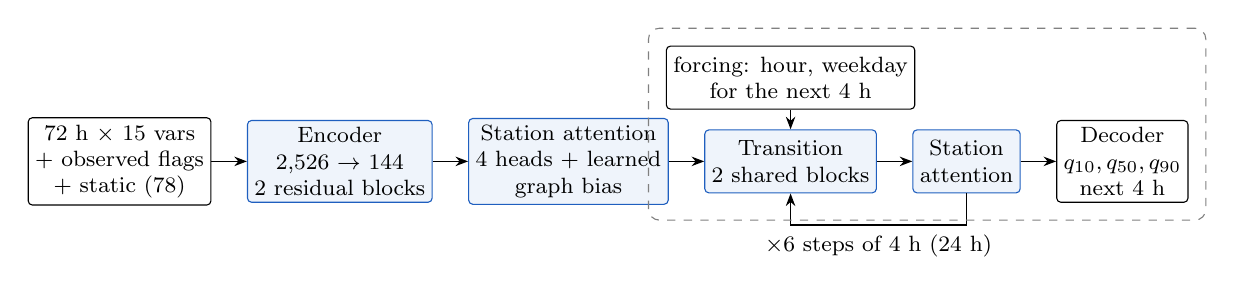
\begin{tikzpicture}[font=\footnotesize, node distance=3mm and 4.5mm,
  box/.style={draw, rounded corners=1.5pt, align=center, inner sep=2.5pt, minimum height=8mm, fill=white},
  hl/.style={box, draw=atlasblue, fill=atlasblue!7},
  arr/.style={-{Stealth[length=1.6mm]}, semithick}]
\node[box] (in) {72 h $\times$ 15 vars\\+ observed flags\\+ static (78)};
\node[hl, right=of in] (enc) {Encoder\\2,526 $\to$ 144\\2 residual blocks};
\node[hl, right=of enc] (att) {Station attention\\4 heads + learned\\graph bias};
\node[hl, right=of att] (tr) {Transition\\2 shared blocks};
\node[hl, right=of tr] (att2) {Station\\attention};
\node[box, right=of att2] (dec) {Decoder\\$q_{10}, q_{50}, q_{90}$\\next 4 h};
\node[box, above=2.5mm of tr] (f) {forcing: hour, weekday\\for the next 4 h};
\draw[arr] (in) -- (enc); \draw[arr] (enc) -- (att); \draw[arr] (att) -- (tr); \draw[arr] (tr) -- (att2);
\draw[arr] (att2) -- (dec); \draw[arr] (f) -- (tr);
\draw[arr] (att2.south) -- ++(0,-4mm) -| node[pos=0.25, below] {$\times 6$ steps of 4 h (24 h)} (tr.south);
\node[draw=gray, dashed, rounded corners, fit=(tr)(att2)(dec)(f), inner sep=2.2mm] {};
\end{tikzpicture}}
\caption{\textbf{Atlas} (967,632 parameters, width 144). The encoder and spatial engine run once; the transition,
attention and decoder run six times, each step adding the next four hours of forcing. The decoder starts at zero, so an
untrained Atlas forecasts persistence; quantiles are offsets from the last observation that cannot cross.}
\label{fig:atlas}
\end{figure}

\paragraph{Atlas.} For every station of a network, Atlas reads 72 hours of 15 channels with observed flags. The four
pollutant targets are divided by the station's own mean over the past week, so a model trained in Kerala can read
Delhi; the other channels are standardised per network. A static summary (78 numbers: daily \pmtf{} means of the last
14 days, the value one week before each forecast hour, the log scale) is appended. The flattened input (2,526 numbers)
is projected to a 144-wide state and passed through two residual blocks (LayerNorm, linear to 288, GELU, linear).
Stations are then mixed by multi-head attention~\citep{vaswani2017attention} whose logits carry a bias computed from
each station pair's edge weight; each station links to the six stations whose daily \pmtf{} co-moves most with its own
(never-trained stations are linked using the validation period). The 24 forecast hours are produced in six latent
steps of four hours: the state absorbs that block's forcing (hour of day, day of week), passes two shared residual
blocks, is mixed again across stations and decoded (Fig.~\ref{fig:atlas}). Training minimises the pinball loss
(weight 1.0 for \pmtf{}, 0.1 for other pollutants, 0.05 for weather) plus a reconstruction loss on 0--40\% randomly
hidden input cells, with AdamW~\citep{loshchilov2019adamw}; full settings are in Appendix~\ref{app:hparams}.

\paragraph{Recipe: pre-train on other cities, then adapt.} \emph{Atlas v1.3}, our Delhi model, is pre-trained on the 13
networks other than Delhi (226 stations, 144,671 windows, ending two years before Delhi's validation period), then
continues on all of Delhi's history at 0.3 times the learning rate. Three seeds are averaged. \emph{Atlas-India}
is the same architecture trained on all 14 networks at once.

\paragraph{Atlas-W.} To ask how much of the problem a far smaller model with a physical prior can capture, Atlas-W
replaces the window with a per-variable summary (last observed value, 6/24/72-hour means relative to it, observed
share, any-value flag) and forecasts by stepping the variables themselves, hour by hour, in transport form:
\begin{equation}
x_{t+1} = x_t + k_t\,(x^{*}_t - x_t) + \kappa\,\big(\bar{x}^{\mathrm{nbr}}_t - x_t\big),
\label{eq:atlasw}
\end{equation}
where $\bar{x}^{\mathrm{nbr}}$ is the row-normalised mean over graph neighbours. The network outputs only the
equilibrium $x^*_t$, the relaxation rate $k_t\in(0,1)$ (sources, sinks, dilution), the exchange rate
$\kappa\in(0,0.5)$ and the quantile spread. Rates start near zero, so an untrained Atlas-W is persistence. At width 32
it has 14,043 parameters.

\paragraph{Opponents.} TSFMs are run zero-shot as released on exactly the same windows, with 512 hours of each
station's own \pmtf{} history (gaps forward-filled): TimesFM~2.5 (200M)~\citep{timesfm25}, Chronos-2
(120M)~\citep{ansari2025chronos2}, Chronos-Bolt (205M)~\citep{chronosbolt}, Moirai~2.0 small (11M)~\citep{moirai2},
TiRex (35M)~\citep{auer2025tirex} and Granite TTM~r2 (0.8M)~\citep{ekambaram2024ttm}. CAMS~\citep{inness2019cams} is
scored from its archived forecasts at the nearest grid cell, raw and with a 30-day local bias correction.

% =================================================================================================================
\section{Results}
\label{sec:results}

\subsection{All of India: the clean test}
\label{sec:india}

\begin{table}[t]
\caption{\textbf{All-India league} (14 networks, 263 stations, 725 windows per network, \pmtf{} MAE in \pmu, next
24 h). Three Atlas-India seeds averaged; every entry calibrated on each network's validation windows. No model choice
used this test period. Last column: relative MAE difference and Diebold--Mariano $p$, trained / never-trained.}
\label{tab:india}
\centering\small
\resizebox{\linewidth}{!}{%
\begin{tabular}{lcccc l}
\toprule
Entry & \trk{s} MAE & \trk{u} MAE & MAE@1h & MAE@24h & Atlas-India against it \\
\midrule
\textbf{Atlas-India} (0.97M) & \textbf{20.99} & \textbf{20.86} & 9.55 & \textbf{23.88} & -- \\
TimesFM 2.5 (200M), zero-shot & 22.35 & 21.93 & \textbf{9.54} & 25.16 & $-6.07\%$ ($p{=}2{\times}10^{-20}$) / $-4.84\%$ ($p{=}4{\times}10^{-11}$) \\
Same hour yesterday & 29.86 & 29.30 & 29.48 & 29.68 & $-29.7\%$ / $-28.8\%$ \\
Last observed value & 32.01 & 31.13 & 11.65 & 28.36 & $-34.4\%$ / $-33.0\%$ \\
\bottomrule
\end{tabular}}
\end{table}

\begin{figure}[t]
\centering
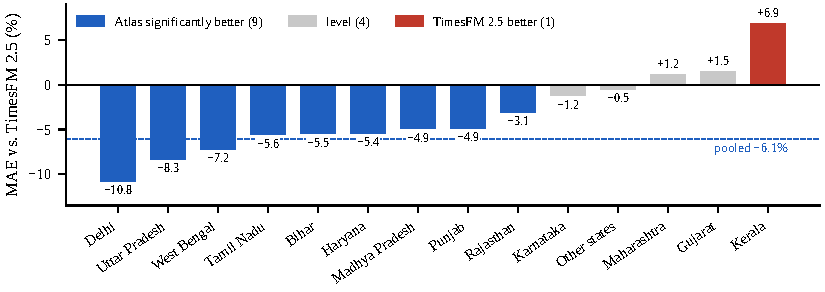
\includegraphics[width=\linewidth]{figures/india_networks.pdf}
\caption{\textbf{Network by network} (trained stations): Atlas-India's MAE relative to TimesFM~2.5. Atlas is
significantly better in 9 networks, level in 4 and worse in Kerala (7 stations, mean \pmtf{} 43~\pmu).}
\label{fig:india}
\end{figure}

One set of Atlas weights beats TimesFM~2.5 across India on both tracks (Table~\ref{tab:india}). Because no Atlas
version was selected or tuned on this test period, this is our cleanest comparison. The gains are largest where
pollution is highest (Delhi $-10.8\%$, Uttar Pradesh $-8.3\%$, Fig.~\ref{fig:india}); the one significant loss is
Kerala, the cleanest network. The two models are level one hour ahead, when both start from the last measurement;
Atlas's lead appears from 6 to 24 hours. Error at never-trained stations (20.86) is no higher than at trained ones
(20.99), and the 80\% intervals contain 78--79\% of measurements.

\subsection{Delhi: a league against every scorable opponent}
\label{sec:delhi}

\begin{table}[t]
\caption{\textbf{Delhi league} (39 stations, 725 windows over 182 days, \pmtf{} next 24 h, MAE in \pmu). Every entry
calibrated on validation; three seeds averaged for our models. Verdicts by the pre-registered rule (both tracks
significant, Diebold--Mariano with a day-block bootstrap); every Atlas~v1.3 comparison below has $p<10^{-3}$ on both
tracks.}
\label{tab:delhi}
\centering\small
\setlength{\tabcolsep}{4.2pt}
\resizebox{\linewidth}{!}{%
\begin{tabular}{l r cc ccc l}
\toprule
Entry & Params & \trk{s} MAE & \trk{u} MAE & RMSE & QL & Cov$_{80}$ & Atlas v1.3 against it (\trk{s} / \trk{u}) \\
\midrule
\textbf{Atlas v1.3} (ours) & 0.97M & \textbf{28.91} & \textbf{25.56} & \textbf{52.82} & \textbf{9.55} & 79 & -- \\
Atlas, other cities only, no Delhi data & 0.97M & 29.98 & 26.11 & -- & 9.92 & 80 & -- \\
Moirai 2.0 R small & 11M & 30.50 & 26.84 & 54.99 & 10.10 & 79 & beats ($-5.2\%$ / $-4.8\%$) \\
TiRex & 35M & 30.73 & 27.09 & 55.34 & 10.10 & 79 & beats ($-5.9\%$ / $-5.7\%$) \\
TimesFM 2.5 & 200M & 30.83 & 27.10 & 55.52 & 10.15 & 78 & beats ($-6.2\%$ / $-5.7\%$) \\
Chronos-2 & 120M & 31.17 & 27.41 & 55.81 & 10.23 & 79 & beats ($-7.3\%$ / $-6.8\%$) \\
Chronos-Bolt & 205M & 31.35 & 27.94 & 56.00 & 10.26 & 79 & beats ($-7.8\%$ / $-8.5\%$) \\
Atlas-W v1 (ours) & 14K & 31.44 & 27.48 & 55.99 & 10.35 & 80 & beats ($-8.0\%$ / $-7.0\%$) \\
Granite TTM r2 & 0.8M & 31.63 & 27.79 & 55.12 & 12.14 & 69 & beats ($-8.6\%$ / $-8.0\%$) \\
CAMS + 30-day bias correction & -- & 41.03 & 38.32 & 65.54 & 14.35 & 76 & beats ($-29.0\%$ / $-32.5\%$) \\
CAMS, archived forecast & -- & 62.86 & 53.53 & 97.71 & 22.66 & 70 & beats ($-53.7\%$ / $-51.7\%$) \\
\bottomrule
\end{tabular}}
\end{table}

\begin{figure}[t]
\centering
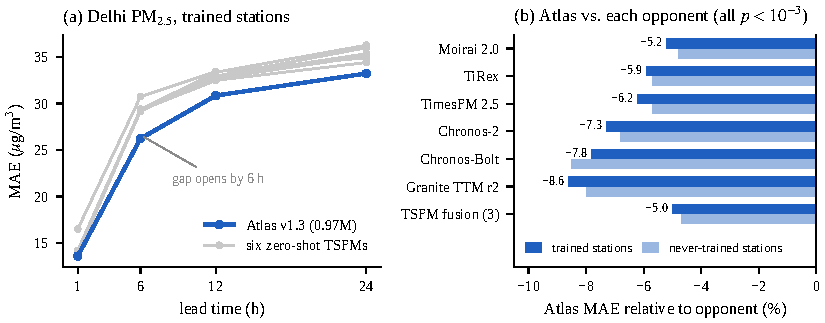
\includegraphics[width=\linewidth]{figures/delhi_league.pdf}
\caption{\textbf{Delhi.} (a) MAE by lead time: all models start near the last measurement; Atlas's advantage opens by
6 hours, when the day's build-up or clearing must be forecast, and holds to 24 hours. (b) Atlas~v1.3's MAE relative to
each opponent on both tracks; the TSFM fusion is an optimised weighted average of TimesFM~2.5, Chronos-2 and
Chronos-Bolt.}
\label{fig:delhi}
\end{figure}

Atlas~v1.3 beats every TSFM we could run, on both tracks, by 5.2--8.6\% (Table~\ref{tab:delhi}, Fig.~\ref{fig:delhi}).
The pinball loss gives the same verdicts ($-5.9\%$ / $-5.4\%$ against TimesFM~2.5), so the gain is not only in the
median. It also beats an online-weighted fusion of TimesFM~2.5, Chronos-2 and Chronos-Bolt (30.43 / 26.82)
by 5.0\% / 4.7\%. TimesFM~3.0 in multivariate mode scored 29.95 / 26.16 on the same windows, 3.5\% / 2.3\% worse than
Atlas by number; its forecasts were not in the tested assembly, so we draw no verdict. Atlas also beats CAMS by
29--54\%; at station scale the 0.4$^\circ$ global chemistry forecast is biased high, and a local correction removes only
part of that.

\paragraph{Atlas adds information the TSFMs lack.} An online fusion of Atlas with TimesFM~2.5, Chronos-2 and
Chronos-Bolt (weights re-chosen daily from the trailing 30 days) scores 28.57 / 25.14, beating Atlas alone
($-1.2\%$, $p{=}0.018$ / $-1.6\%$, $p{=}6{\times}10^{-4}$). Against the same fusion without Atlas it is 6.1\% / 6.3\%
better ($p<10^{-6}$), and Atlas carries 0.63 of the fused weight on average (TimesFM~2.5: 0.20).

\paragraph{Weather as a by-product.} Atlas forecasts each station's temperature, humidity and wind only because it
reads them (loss weight 0.05). Against the archived runs of ECMWF IFS and AIFS, DWD ICON and NOAA GFS it wins on all
three variables. After a local bias correction it is level with AIFS on temperature (1.14~$^\circ$C), loses to AIFS
on humidity at never-trained stations ($+13.4\%$), and wins on wind, where the low readings of the boards' wind
sensors make the verdict more about the sensors than the models (Appendix~\ref{app:weather}). We make no claim about
weather skill.

\subsection{What made the difference: related data, not scale}
\label{sec:transfer}

\begin{table}[t]
\caption{\textbf{Atlas versions on Delhi.} Each changed one thing and was chosen over the last on validation only.
Single-model columns: mean and range over seeds, trained stations.}
\label{tab:versions}
\centering\small
\resizebox{\linewidth}{!}{%
\begin{tabular}{llccl}
\toprule
Version & Change & Single model, \trk{s} & Ensemble \trk{s} / \trk{u} & vs.\ TimesFM 2.5 \\
\midrule
v1.0 & 16 months of Delhi (3,673 windows) & -- & 33.42 / 29.07 & loses \\
v1.1 & all Delhi history since 2018 (19,082 windows) & 31.61 & 30.26 / 26.62 & level \\
v1.2 & eight seeds, full schedule & 32.65 (31.37--33.87) & 30.39 / 26.59 & level \\
v1.3, before adaptation & 13 other networks only, no Delhi data & 30.52 (30.22--30.67) & 29.98 / 26.11 & level$^\dagger$ \\
v1.3 & then all Delhi history & 29.81 (29.74--29.93) & \textbf{28.91 / 25.56} & beats \\
\bottomrule
\multicolumn{5}{l}{\footnotesize $^\dagger$ $-2.75\%$ ($p{=}0.054$) / $-3.64\%$ ($p{=}0.011$): better at never-trained stations, not significant at trained ones.}
\end{tabular}}
\end{table}

Table~\ref{tab:versions} traces how Atlas came to beat the TSFMs. Five times more Delhi data (v1.1) brought it level;
eight seeds and the full schedule (v1.2) changed nothing (the weights after the last step were worse on validation than
the early-stopped ones in all eight seeds). What changed the verdict was data from \emph{other} cities: the model
pre-trained on 13 networks, with no Delhi data at all, was already level with TimesFM~2.5 on Delhi, and adapting it
made the win decisive. Pre-training also stabilised training: the spread of single-model test error across seeds fell
from 2.5~\pmu{} (v1.2) to 0.2 (v1.3). Before the run we predicted the single-model error from the data-scaling slope
measured on Delhi: 29.2 if another state's window is worth a Delhi window, 31.5 if it is worth a tenth and 32.4 if it is
worth nothing. The measured 29.81 lies between the first two, nearer the first.

% ---- T1 (pre-registered 2026-11-14, README "ICML programme, T1"): enable when score_threshold.py has run ----
\iffalse
\paragraph{The transfer threshold function.} How much local history does pre-training replace? On the four
leave-one-network-out networks we give Atlas only the most recent $B\in\{0,\tfrac12,1,2,4,8,16,\text{all}\}$ months
of a network's data. The network is treated as if it had started measuring then: every earlier value is removed,
and scaling and graph links are recomputed from what remains. Atlas is then trained from random weights (scratch) or
adapted from the 13-network checkpoint (pre). With $r$ the test MAE relative to TimesFM~2.5, we fit the scratch law
$r=c_X+a\,n^{-\alpha}$ ($n$ = local training windows) and define the effective data transferred,
$D_T(n)=n_{\mathrm{eq}}-n$, where the scratch law reaches the pre-trained model's $r$ at $n_{\mathrm{eq}}$
\citep{hernandez2021scaling}. TABLE/FIGURE: r vs months, both arms, four networks; n* per arm; fitted $\alpha$, $k$,
$\gamma$. RULE: pre lowers n* on $\ge3$ of 4 networks -- RESULT.
\fi

\subsection{Atlas-W: how small can the model be?}
\label{sec:atlasw}

\begin{figure}[t]
\centering
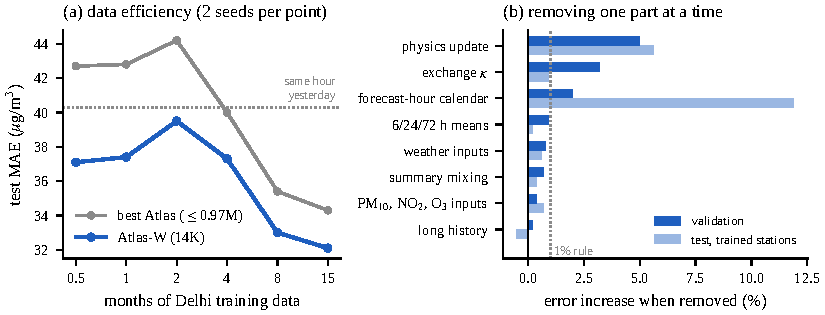
\includegraphics[width=\linewidth]{figures/atlasw.pdf}
\caption{\textbf{Atlas-W.} (a) Test MAE against months of Delhi training data, two seeds per point: Atlas-W
(14,043 parameters) is 6--13\% below the best Atlas size at every budget and beats same-hour-yesterday from two weeks of
data (Atlas needs four months). Both curves rise at two months because the most recent months before validation are a
hard season for the winter test. (b) Error increase when one part is removed (two seeds, 16 months); the dotted line is
the pre-registered 1\% rule on validation.}
\label{fig:atlasw}
\end{figure}

\paragraph{Data efficiency.} Trained on the last 0.5 to 15 months of Delhi data, Atlas-W has lower test error than
every Atlas size (up to 0.97M parameters) at every budget, by 6--13\% (Fig.~\ref{fig:atlasw}a). With all 16 months it
scores 31.97 / 27.43 against 33.42 / 29.07 for Atlas~v1.0 on the same data.

\paragraph{What carries the accuracy.} We removed one part at a time; a part earns its place if removing it raises
validation error by at least 1\% (rule fixed in advance). Three parts do (Fig.~\ref{fig:atlasw}b): the update of
Eq.~\ref{eq:atlasw} (replaced by a direct per-hour output, validation $+5.0\%$; on test the full model wins by
$5.6\%$ / $6.5\%$, $p<10^{-5}$), the exchange term $\kappa$ ($+3.2\%$) and the calendar of the forecast hours
($+2.0\%$ on validation, $+11.9\%$ on test). Weather inputs, the other pollutants, the 6/24/72-hour means, the long
history and summary mixing each change validation error by less than 1\%. Size does not matter: at full data,
widths 16 to 128 (6,139 to 115,227 parameters) all score between 32.1 and 32.6, and a fitted threshold function
$e(N,P)$ puts essentially no weight on $P$ (Appendix~\ref{app:atlasw}).

\paragraph{Limits.} Trained by the v1.3 recipe, Atlas-W reaches 31.44 / 27.48 (Table~\ref{tab:delhi}). We had
predicted 29.5--31.0; the recipe that cut Atlas's error by 13.5\% cut Atlas-W's by 1.7\%. Atlas beats it by 8.0\% /
7.0\%, and by number it sits 0.6--0.9 behind Moirai~2.0 and TimesFM~2.5 on trained stations (not tested directly).
Its pre-trained weights, which never saw a Delhi station, score 31.91 / 27.63, as well as Atlas-W trained on 16 months
of Delhi: transfer is complete, but the model stops near 31.5~\pmu{} whatever its data or size. Its form, not its
scale, is what moves it.

% =================================================================================================================
\section{Pre-registered negative results}
\label{sec:negative}

\paragraph{A lockdown counterfactual failed its validity gate.} A version of Atlas with every pollutant input removed
simulated Delhi's \pmtf{} ``as if emissions continued'' from weather, calendar and each station's usual level. The
rule required no gap on the same dates of 2019 (a placebo) \emph{and} in the three weeks before the 2020 lockdown. The
placebo passed (bias $+0.1\%$), but measured \pmtf{} was already 20.7\% below the simulation before any restriction;
adding ERA5~\citep{hersbach2020era5} rain and boundary-layer height cut the gap only to 16.5\%. The simulated phase-1
drop ($-52\%$) is therefore not claimed as a lockdown effect (Appendix~\ref{app:lockdown}); the method could not
separate the lockdown from a March already cleaner than any year it had seen, consistent with the difficulty reported
by~\citep{shi2021lockdown}.

\paragraph{A data-scaling law did not transfer out of domain.} A law for how error falls with data, fitted on 46
Indian learning curves and frozen, predicted the full-data error of 22 electricity, traffic, solar and transformer
networks from two-month pilots with median error 3.8\% (against 12.2\% for a power law fitted per network). It was
closer in 16 of 22 networks where the rule required 17 ($p{=}0.053$), so the transfer is not claimed.

\paragraph{Continuous retraining made the model worse.} Replaying July--December 2025, a weekly fine-tune of the
deployed Atlas, kept only if it beat the old weights on the latest week, raised error to 30.39 / 26.94 ($+5.1\%$ /
$+5.4\%$, $p<10^{-3}$), worst in November. The gate accepted 51 of 78 updates, about what noise alone passes, and the
updates eroded what pre-training knew about winter. A daily bias-and-band correction was level ($+0.6\%$, $p{=}0.59$).

% =================================================================================================================
\section{Discussion, limitations and conclusion}
\label{sec:conclusion}

\paragraph{Why a small model can win here.} We did not ablate Atlas itself, so these are hypotheses consistent with
the evidence, not findings. (i)~\emph{Information, not capacity.} The TSFMs read one station's \pmtf{} alone; Atlas
reads 15 variables at every station of the network. The one TSFM we also ran multivariately improved when given more
than the target series (TimesFM~3.0: 30.31 univariate, 29.95 multivariate). (ii)~\emph{A regular cycle learned from
many stations.} The gap opens at 6 hours, when the day's build-up or clearing must be forecast, and in Atlas-W the
calendar of the forecast hours is the most consequential input ($+11.9\%$ on test when removed). (iii)~\emph{Domain
exposure.} Atlas-W's error is insensitive to a 19-fold change in parameters, while Atlas's fell by 13.5\% when it was
pre-trained on other Indian cities. Together these suggest that what holds the TSFMs back on this task is what they
see, not their size.

\paragraph{Limitations.} All results are \pmtf{} at Indian stations; nothing here shows that Atlas works for other
variables, regions or horizons beyond 24 hours. Both test periods contain the north-Indian winter. Delhi's test period
was reused across versions, so the Delhi gain is provisional until the leave-one-network-out repetition of the v1.3
recipe succeeds elsewhere; the all-India win is on clean data but uses a model trained on all networks at once.
The TSFMs were run zero-shot and univariate, as released; fine-tuned or multivariate variants could do better.
TimesFM~3.0, Sundial, Toto, the graph architectures and AI weather models run by us had not been scored when this
paper was written. Operational Indian forecasts~\citep{yadav2025aqews} publish no archive at these stations; a forward
test is the comparison that remains. The architecture admits interventions through its forcing, but the only
counterfactual test failed, so we make no world-model claim.

\paragraph{Conclusion.} A model of under one million parameters, trained only on station measurements, forecasts
Indian \pmtf{} significantly better than six zero-shot foundation models with up to 205M parameters, at stations it was
trained on and at stations it never saw, and on a test period that no choice touched. The deciding factor was related
data from other cities, not size: a 14K-parameter model with a physical update is more data-efficient still, and
size made no difference to it. Foundation models are not made redundant (fused with Atlas they still lower the
error), but on this domain a small model with the right data and structure is the stronger forecaster.

\ifpreprint
\paragraph{Code and data.} Code, every rule, prediction and result in the order written, and the notebooks that produced
every number: \url{https://github.com/paradoxailab/paradox-world-model} (branch \texttt{atlas-v0.1}). No data, weights
or keys are stored; all data are public and rebuilt by the repository's scripts.
\else
\paragraph{Code and data.} Code, the time-stamped rules and the notebooks that produced every number are in a public
repository whose link is withheld for review; an anonymised copy is provided as supplementary material.
\fi

\bibliographystyle{plainnat}
\bibliography{refs}

% =================================================================================================================
\newpage
\appendix

\section{Data details}
\label{app:data}

\begin{table}[H]
\caption{All-India networks: stations (never-trained in brackets) and mean \pmtf{} over the test period.}
\centering\small
\begin{tabular}{lcc@{\hspace{2.2em}}lcc}
\toprule
Network & Stations & Mean \pmtf{} & Network & Stations & Mean \pmtf{} \\
\midrule
Uttar Pradesh & 40 (8) & 77 & West Bengal & 14 (3) & 75 \\
Delhi & 37 (7) & 140 & Bihar & 12 (2) & 121 \\
Haryana & 30 (6) & 86 & Rajasthan & 10 (2) & 63 \\
Maharashtra & 27 (5) & 74 & Gujarat & 9 (2) & 67 \\
Karnataka & 24 (5) & 34 & Tamil Nadu & 9 (2) & 42 \\
Other states & 22 (4) & 55 & Punjab & 8 (2) & 65 \\
Madhya Pradesh & 14 (3) & 57 & Kerala & 7 (1) & 43 \\
\bottomrule
\end{tabular}
\end{table}

\textbf{Sources.} Delhi 2024--25 from OpenCity's Delhi Hourly Air Quality Reports~\citep{opencity}; earlier Delhi
history and all-India data from the public Kaggle dataset \emph{Time Series Air Quality Data of India
(2010--2023)}~\citep{kaggleaq}, both copies of CPCB station exports~\citep{cpcb}; ERA5 through the Open-Meteo
archive~\citep{openmeteo} for the lockdown test only. \textbf{Eligibility (all-India).} 453 stations from 2017 to March
2023; a station enters if it reports \pmtf{} on at least 50\% of test hours and 12.5\% of training hours.
\textbf{Cleaning.} Timestamps are moved to Indian time, detecting files written in UTC from the hour of the
solar-radiation peak; values that are not numbers, negative (except temperature) or above physical ceilings become
missing; a pollutant stuck at one value for 24 hours becomes missing. \textbf{Input fault, found before scoring.} In
Gujarat and Kerala the only pressure sensor, and in Punjab the only temperature sensor, sat at a never-trained station
and entered unscaled; such variables are now dropped as inputs in that network. Saved weights were reused and no
trained-station forecast changed (largest change $<10^{-4}$~\pmu); both scorings are in the repository.

\section{Model and training settings}
\label{app:hparams}

\begin{table}[H]
\caption{Atlas settings (identical for Delhi and all-India models unless stated).}
\centering\small
\begin{tabularx}{\linewidth}{@{}lX@{}}
\toprule
Width / parameters & 144 / 967,632 \\
Input & 72 h $\times$ 15 channels + flags, static summary of 78 numbers (2,526 inputs per station) \\
Encoder & linear to 144, 2 residual blocks (LayerNorm, 144$\to$288, GELU, 288$\to$144) \\
Spatial engine & 4-head attention, learned bias from (edge weight, self-loop, edge) per pair; 6 neighbours by \pmtf{} co-movement \\
Dynamics & 6 steps of 4 h; forcing = hour-of-day and weekday (sin/cos); 2 shared residual blocks per step \\
Output & median = last value + learned correction; $q_{10},q_{90}$ via softplus offsets; pollutants $\geq 0$ \\
Loss & pinball (weights 1.0 \pmtf{}, 0.1 other pollutants, 0.05 weather) + 0.2 $\times$ reconstruction of 0--40\% hidden cells \\
Optimiser & AdamW, lr $10^{-3}$, weight decay $10^{-4}$, 100 warm-up steps, cosine to 10\%, clip 1.0 \\
Batch & 16 windows, all trained stations of one network \\
Selection & best validation checkpoint (early stopping), chosen over last step by rule \\
All-India & 60,000 steps on 158,893 windows sampled by network size; 3 seeds \\
Delhi v1.3 & pre-train as all-India without Delhi (144,671 windows); then all Delhi history at 0.3 $\times$ lr; 3 seeds \\
\midrule
Atlas-W & width 32, 14,043 parameters; inputs: 6 summary features $\times$ 15 variables + the 78 static numbers; \\
 & one residual block, one neighbour mixing, heads for $x^*$, $k$, $\kappa$, spread; rate biases start at $-4$ \\
\bottomrule
\end{tabularx}
\end{table}

\section{Weather by-product}
\label{app:weather}

\begin{table}[H]
\caption{Atlas~v1.3's weather channels against global models' runs issued the day before each forecast hour, at the
CPCB stations measuring each variable (temperature 26, humidity 31, wind 29). MAE \trk{s} / \trk{u}. NOAA AIGFS and DWD
AICON have no public archive at these dates.}
\centering\small
\resizebox{\linewidth}{!}{%
\begin{tabular}{lcccl}
\toprule
Variable & Atlas v1.3 & Best raw model & Best bias-corrected & Atlas against best bias-corrected \\
\midrule
Temperature ($^\circ$C) & 1.14 / 1.28 & AIFS 1.99 / 2.33 & AIFS 1.28 / 1.35 & $-10.8\%$ ($p{=}0.001$) / $-5.0\%$ ($p{=}0.17$): level \\
Humidity (\%) & 5.64 / 6.57 & AIFS 8.69 / 8.20 & AIFS 5.70 / 5.47 & $-2.6\%$ ($p{=}0.36$) / $+13.4\%$ ($p{<}10^{-5}$): loses \\
Wind speed (m/s) & 0.38 / 0.32 & ICON 0.89 / 0.76 & ICON 0.60 / 0.51 & $-35.8\%$ / $-35.1\%$: beats \\
\bottomrule
\end{tabular}}
\end{table}

Most of Atlas's edge is at short leads (temperature MAE 0.43~$^\circ$C at 1 h against 1.28 for corrected AIFS;
1.10 against 1.27 at 24 h); at 24 h corrected AIFS is better on humidity (5.65 against 6.02).

\section{Atlas-W details}
\label{app:atlasw}

\begin{table}[H]
\caption{Atlas-W test MAE (trained stations, two seeds) by width and training data. With all data, sizes spanning
19$\times$ lie within 0.5~\pmu. The fitted $e(N,P)=e_0+aN^{-\alpha}+bP^{-\beta}$ over 48 runs gives $b=0.0016$,
$\beta=2.9$ (no weight on $P$), $\alpha=0.045$, misfit $\times1.046$.}
\centering\small
\begin{tabular}{lrcccccc}
\toprule
Width & Params & 0.5 mo & 1 mo & 2 mo & 4 mo & 8 mo & all (15 mo) \\
\midrule
16 & 6,139 & 35.8 & 38.4 & 40.6 & 35.7 & 32.8 & 32.4 \\
32 & 14,043 & 37.1 & 37.4 & 39.5 & 37.3 & 33.0 & 32.1 \\
64 & 37,531 & 37.9 & 37.4 & 39.2 & 36.6 & 33.4 & 32.3 \\
128 & 115,227 & 37.6 & 37.7 & 37.7 & 35.8 & 34.9 & 32.6 \\
\midrule
Best Atlas ($\le$0.97M) & & 42.7 & 42.8 & 44.2 & 40.0 & 35.4 & 34.3 \\
\bottomrule
\end{tabular}
\end{table}

\begin{table}[H]
\caption{Atlas-W removals (two seeds, width 32, 16 months). Full model: validation 20.49, test 32.03 / 27.44.
``Full against it'': Diebold--Mariano on test, \trk{s} / \trk{u} (negative = full model better).}
\centering\small
\resizebox{\linewidth}{!}{%
\begin{tabular}{lccl l}
\toprule
Removed & Val.\ change & Test \trk{s} / \trk{u} & Full against it & Earns its place \\
\midrule
Update of Eq.~\ref{eq:atlasw} (direct output) & $+5.0\%$ & 33.92 / 29.34 & $-5.6\%$ / $-6.5\%$ ($p<10^{-5}$) & yes \\
Exchange $\kappa$ & $+3.2\%$ & 32.32 / 27.78 & $-0.9\%$ (n.s.) / $-1.2\%$ ($p{=}0.047$) & yes \\
Calendar of forecast hours & $+2.0\%$ & 36.35 / 30.75 & $-11.9\%$ / $-10.8\%$ ($p<10^{-7}$) & yes \\
6/24/72 h means & $+0.9\%$ & 32.10 / 27.61 & level / level & no \\
Weather inputs & $+0.8\%$ & 32.23 / 27.75 & level / $-1.1\%$ & no \\
Summary mixing & $+0.7\%$ & 32.15 / 27.66 & level / $-0.8\%$ & no \\
PM$_{10}$, NO$_2$, O$_3$ inputs & $+0.4\%$ & 32.24 / 27.57 & $-0.7\%$ / $-0.5\%$ & no \\
Long history (daily means, week-ago value) & $+0.2\%$ & 31.89 / 27.42 & level / level & no \\
\bottomrule
\end{tabular}}
\end{table}

\section{Lockdown counterfactual}
\label{app:lockdown}

\begin{table}[H]
\caption{Measured \pmtf{} against the simulated business-as-usual, Delhi. Test 1b adds ERA5 rain and boundary-layer
height. The gate required both the placebo and the pre-lockdown window to show no gap; the second failed in both tests.}
\centering\small
\resizebox{\linewidth}{!}{%
\begin{tabular}{lcccc}
\toprule
Window & Measured (\pmu) & Simulated, test 1 & Gap, test 1 & Gap, test 1b \\
\midrule
25 Mar -- 31 May 2019 (placebo) & 88.1 & 88.1 & $+0.1\%$ & $+6.7\%$ \\
1 -- 21 Mar 2020 (before lockdown) & 67.1 & 84.6 & $-20.7\%$ & $-16.5\%$ \\
25 Mar -- 14 Apr 2020 (lockdown phase 1) & 39.4 & 82.3 & $-52.1\%$ & $-48.7\%$ \\
\bottomrule
\end{tabular}}
\end{table}

The added reanalysis explained 12--21 March 2020, the wettest days (gap $-4.1\%$), but not 1--11 March ($-26.2\%$),
which came before any restriction. A replication on different hardware gave the same verdicts.

\section{Continuous updating}

\begin{table}[H]
\caption{Atlas-Live replay, July--December 2025 (Delhi, MAE \trk{s} / \trk{u}).}
\centering\small
\resizebox{\linewidth}{!}{%
\begin{tabular}{lccl}
\toprule
Layer & \trk{s} & \trk{u} & Against the frozen model \\
\midrule
Frozen Atlas v1.3 & 28.91 & 25.56 & -- \\
+ daily bias and band correction (30 days) & 29.08 & 25.79 & level ($+0.6\%$, $p{=}0.59$ / $+0.9\%$, $p{=}0.39$) \\
+ weekly gated fine-tune & 30.39 & 26.94 & loses ($+5.1\%$, $p{=}0.0009$ / $+5.4\%$, $p{=}0.0004$) \\
\bottomrule
\end{tabular}}
\end{table}

By month (trained stations, frozen / daily / weekly): October 32.0 / 31.8 / 33.4, November 48.6 / 49.9 / 54.2,
December 53.9 / 53.3 / 54.8; July--September all within 0.5~\pmu.

\section{Compute and reproducibility}

Every experiment ran on free tiers: Kaggle CPU sessions (Atlas seeds 19--100 minutes each; Atlas-W pre-training
41--44 minutes; the longest single run 666 minutes) and a T4 GPU for TimesFM~2.5 on all of India (44 minutes); Moirai~2.0,
TiRex and TTM ran on CPU (5.8, 284.9 and 0.8 minutes). Each scoring run first reproduces the recorded Atlas~v1.3 score
(28.91 / 25.56) and the opponents' recorded numbers before adding new entries. Licences: TimesFM~2.5, Chronos-2,
Chronos-Bolt and Granite TTM are Apache-2.0; Moirai~2.0 (CC-BY-NC-4.0), TiRex (NXAI community licence) and TimesFM~3.0
(non-commercial) were used for evaluation only and never as components of our models.

% =================================================================================================================
\newpage
\section*{NeurIPS Paper Checklist}

\begin{enumerate}[leftmargin=1.5em]
\item \textbf{Claims.} Do the abstract and introduction accurately reflect the paper's contributions and scope?
  \textbf{[Yes]} Each contribution is stated with its test; provisional and failed claims are labelled (\S\ref{sec:intro}, \S\ref{sec:negative}).
\item \textbf{Limitations.} \textbf{[Yes]} \S\ref{sec:conclusion}: one country, one target, winter-dominated tests, Delhi test reuse, zero-shot opponents, unscored opponents, no world-model claim.
\item \textbf{Theory assumptions and proofs.} \textbf{[NA]} No theoretical results.
\item \textbf{Experimental result reproducibility.} \textbf{[Yes]} Data sources, cleaning, splits, architecture, settings and protocol are in \S\ref{sec:data}--\ref{sec:models} and Appendices~\ref{app:data}--\ref{app:hparams}.
\item \textbf{Open access to data and code.} \textbf{[Yes]} All data are public; code, rules and notebooks are in a public repository (anonymised for review).
\item \textbf{Experimental setting/details.} \textbf{[Yes]} Appendix~\ref{app:hparams}; selection only on validation by fixed rules.
\item \textbf{Experiment statistical significance.} \textbf{[Yes]} Diebold--Mariano tests with a day-block bootstrap on both tracks for every comparison; seed ranges reported.
\item \textbf{Experiments compute resources.} \textbf{[Yes]} Appendix, ``Compute and reproducibility''.
\item \textbf{Code of ethics.} \textbf{[Yes]} Public environmental data with no personal information.
\item \textbf{Broader impacts.} \textbf{[Yes]} Better station forecasts can support health advisories in highly polluted cities; a wrong forecast could mislead such advisories, so intervals are calibrated and failures reported. The failed counterfactual test is reported so that the model is not used for policy attribution.
\item \textbf{Safeguards.} \textbf{[NA]} No high-risk release.
\item \textbf{Licenses for existing assets.} \textbf{[Yes]} Data sources and model licences are cited and listed; non-commercial models were used for evaluation only.
\item \textbf{New assets.} \textbf{[Yes]} Code and pre-registered rules are documented in the repository; no data or weights are redistributed.
\item \textbf{Crowdsourcing and research with human subjects.} \textbf{[NA]}
\item \textbf{IRB approvals.} \textbf{[NA]}
\item \textbf{Declaration of LLM usage.} \textbf{[Yes]} An LLM-based assistant (Claude, Anthropic) was used to write code, run experiments and draft text. The authors checked and are responsible for all content.
\end{enumerate}

\end{document}
